% Options for packages loaded elsewhere
\PassOptionsToPackage{unicode}{hyperref}
\PassOptionsToPackage{hyphens}{url}
%
\documentclass[
]{article}
\usepackage{amsmath,amssymb}
\usepackage{lmodern}
\usepackage{ifxetex,ifluatex}
\ifnum 0\ifxetex 1\fi\ifluatex 1\fi=0 % if pdftex
  \usepackage[T1]{fontenc}
  \usepackage[utf8]{inputenc}
  \usepackage{textcomp} % provide euro and other symbols
\else % if luatex or xetex
  \usepackage{unicode-math}
  \defaultfontfeatures{Scale=MatchLowercase}
  \defaultfontfeatures[\rmfamily]{Ligatures=TeX,Scale=1}
\fi
% Use upquote if available, for straight quotes in verbatim environments
\IfFileExists{upquote.sty}{\usepackage{upquote}}{}
\IfFileExists{microtype.sty}{% use microtype if available
  \usepackage[]{microtype}
  \UseMicrotypeSet[protrusion]{basicmath} % disable protrusion for tt fonts
}{}
\makeatletter
\@ifundefined{KOMAClassName}{% if non-KOMA class
  \IfFileExists{parskip.sty}{%
    \usepackage{parskip}
  }{% else
    \setlength{\parindent}{0pt}
    \setlength{\parskip}{6pt plus 2pt minus 1pt}}
}{% if KOMA class
  \KOMAoptions{parskip=half}}
\makeatother
\usepackage{xcolor}
\IfFileExists{xurl.sty}{\usepackage{xurl}}{} % add URL line breaks if available
\IfFileExists{bookmark.sty}{\usepackage{bookmark}}{\usepackage{hyperref}}
\hypersetup{
  pdftitle={DDS Case Study 1},
  pdfauthor={Allen Hoskins},
  hidelinks,
  pdfcreator={LaTeX via pandoc}}
\urlstyle{same} % disable monospaced font for URLs
\usepackage[margin=1in]{geometry}
\usepackage{color}
\usepackage{fancyvrb}
\newcommand{\VerbBar}{|}
\newcommand{\VERB}{\Verb[commandchars=\\\{\}]}
\DefineVerbatimEnvironment{Highlighting}{Verbatim}{commandchars=\\\{\}}
% Add ',fontsize=\small' for more characters per line
\usepackage{framed}
\definecolor{shadecolor}{RGB}{248,248,248}
\newenvironment{Shaded}{\begin{snugshade}}{\end{snugshade}}
\newcommand{\AlertTok}[1]{\textcolor[rgb]{0.94,0.16,0.16}{#1}}
\newcommand{\AnnotationTok}[1]{\textcolor[rgb]{0.56,0.35,0.01}{\textbf{\textit{#1}}}}
\newcommand{\AttributeTok}[1]{\textcolor[rgb]{0.77,0.63,0.00}{#1}}
\newcommand{\BaseNTok}[1]{\textcolor[rgb]{0.00,0.00,0.81}{#1}}
\newcommand{\BuiltInTok}[1]{#1}
\newcommand{\CharTok}[1]{\textcolor[rgb]{0.31,0.60,0.02}{#1}}
\newcommand{\CommentTok}[1]{\textcolor[rgb]{0.56,0.35,0.01}{\textit{#1}}}
\newcommand{\CommentVarTok}[1]{\textcolor[rgb]{0.56,0.35,0.01}{\textbf{\textit{#1}}}}
\newcommand{\ConstantTok}[1]{\textcolor[rgb]{0.00,0.00,0.00}{#1}}
\newcommand{\ControlFlowTok}[1]{\textcolor[rgb]{0.13,0.29,0.53}{\textbf{#1}}}
\newcommand{\DataTypeTok}[1]{\textcolor[rgb]{0.13,0.29,0.53}{#1}}
\newcommand{\DecValTok}[1]{\textcolor[rgb]{0.00,0.00,0.81}{#1}}
\newcommand{\DocumentationTok}[1]{\textcolor[rgb]{0.56,0.35,0.01}{\textbf{\textit{#1}}}}
\newcommand{\ErrorTok}[1]{\textcolor[rgb]{0.64,0.00,0.00}{\textbf{#1}}}
\newcommand{\ExtensionTok}[1]{#1}
\newcommand{\FloatTok}[1]{\textcolor[rgb]{0.00,0.00,0.81}{#1}}
\newcommand{\FunctionTok}[1]{\textcolor[rgb]{0.00,0.00,0.00}{#1}}
\newcommand{\ImportTok}[1]{#1}
\newcommand{\InformationTok}[1]{\textcolor[rgb]{0.56,0.35,0.01}{\textbf{\textit{#1}}}}
\newcommand{\KeywordTok}[1]{\textcolor[rgb]{0.13,0.29,0.53}{\textbf{#1}}}
\newcommand{\NormalTok}[1]{#1}
\newcommand{\OperatorTok}[1]{\textcolor[rgb]{0.81,0.36,0.00}{\textbf{#1}}}
\newcommand{\OtherTok}[1]{\textcolor[rgb]{0.56,0.35,0.01}{#1}}
\newcommand{\PreprocessorTok}[1]{\textcolor[rgb]{0.56,0.35,0.01}{\textit{#1}}}
\newcommand{\RegionMarkerTok}[1]{#1}
\newcommand{\SpecialCharTok}[1]{\textcolor[rgb]{0.00,0.00,0.00}{#1}}
\newcommand{\SpecialStringTok}[1]{\textcolor[rgb]{0.31,0.60,0.02}{#1}}
\newcommand{\StringTok}[1]{\textcolor[rgb]{0.31,0.60,0.02}{#1}}
\newcommand{\VariableTok}[1]{\textcolor[rgb]{0.00,0.00,0.00}{#1}}
\newcommand{\VerbatimStringTok}[1]{\textcolor[rgb]{0.31,0.60,0.02}{#1}}
\newcommand{\WarningTok}[1]{\textcolor[rgb]{0.56,0.35,0.01}{\textbf{\textit{#1}}}}
\usepackage{graphicx}
\makeatletter
\def\maxwidth{\ifdim\Gin@nat@width>\linewidth\linewidth\else\Gin@nat@width\fi}
\def\maxheight{\ifdim\Gin@nat@height>\textheight\textheight\else\Gin@nat@height\fi}
\makeatother
% Scale images if necessary, so that they will not overflow the page
% margins by default, and it is still possible to overwrite the defaults
% using explicit options in \includegraphics[width, height, ...]{}
\setkeys{Gin}{width=\maxwidth,height=\maxheight,keepaspectratio}
% Set default figure placement to htbp
\makeatletter
\def\fps@figure{htbp}
\makeatother
\setlength{\emergencystretch}{3em} % prevent overfull lines
\providecommand{\tightlist}{%
  \setlength{\itemsep}{0pt}\setlength{\parskip}{0pt}}
\setcounter{secnumdepth}{-\maxdimen} % remove section numbering
\ifluatex
  \usepackage{selnolig}  % disable illegal ligatures
\fi

\title{DDS Case Study 1}
\author{Allen Hoskins}
\date{6/1/2021}

\begin{document}
\maketitle

\#Intro

Mr.~Doukeris and Mr.~Tennenbaum, according to The Beer Institute on
average the adult 21 and over consumes around 28.2 gallons of beer a
year. Which equates to roughly a six pack of beer per week. During my
analysis of the brewery data, I have found that on average each state
has 11 breweries With the exception of California, Colorado, Michigan,
Texas, and Oregon which contain over 28 breweries each. Colorado not
only contains the most breweries with 47 total but also the biggest ABV
at 12.8\% while Oregon has the most bitter at 138 IBU which ranges from
0 to 140. We suggest that adding an additional breweries to Arizona,
South Carolina, Indiana, and Maine would greatly impact beer sales to
combat the ever growing microbrewery influx. According to the Associated
Press, these states have seen the least amount of population decline of
the the last year. Additions to California, Georgia, New York and Texas
would also be beneficial due those states having a low brewery per 100k,
with populations over 28mm people. While Texas and California have some
of the highest number of breweries in total, they average less than .5
breweries per 100k. IPA's and Ale's consist of more 60\% of the beers
and continue to rise are the most common consumed beer in the United
States. Additions of higher ABV beers such as IPAs to the Western and
Southern Regions and additions of lower IBU beers such as Ales in the
North Central and Northeast would increase sales as these align with the
current selection in the area.

Pertaining to beer classifications that were asked, we can accurately
predict whether a beer is an Ale or an IPA based on the combination of
IBU and ABV at a rate of almost 92\% using a model based off of
comparing similar beer components called k-nearest neighbor. When
comparing to other commonly used models such as Naïve-Bayes it performed
at a significantly better rate.

\hypertarget{code-chunk-1}{%
\section{Code Chunk 1:}\label{code-chunk-1}}

\#\#Reading in Data from supplied CSV files

\begin{Shaded}
\begin{Highlighting}[]
\FunctionTok{library}\NormalTok{(tidyr)}
\FunctionTok{library}\NormalTok{(tidyverse)}
\end{Highlighting}
\end{Shaded}

\begin{verbatim}
## -- Attaching packages --------------------------------------- tidyverse 1.3.1 --
\end{verbatim}

\begin{verbatim}
## v ggplot2 3.3.3     v dplyr   1.0.6
## v tibble  3.1.1     v stringr 1.4.0
## v readr   1.4.0     v forcats 0.5.1
## v purrr   0.3.4
\end{verbatim}

\begin{verbatim}
## -- Conflicts ------------------------------------------ tidyverse_conflicts() --
## x dplyr::filter() masks stats::filter()
## x dplyr::lag()    masks stats::lag()
\end{verbatim}

\begin{Shaded}
\begin{Highlighting}[]
\FunctionTok{library}\NormalTok{(magrittr)}
\end{Highlighting}
\end{Shaded}

\begin{verbatim}
## 
## Attaching package: 'magrittr'
\end{verbatim}

\begin{verbatim}
## The following object is masked from 'package:purrr':
## 
##     set_names
\end{verbatim}

\begin{verbatim}
## The following object is masked from 'package:tidyr':
## 
##     extract
\end{verbatim}

\begin{Shaded}
\begin{Highlighting}[]
\FunctionTok{library}\NormalTok{(dplyr)}
\FunctionTok{library}\NormalTok{(readr)}
\FunctionTok{library}\NormalTok{(knitr)}

\CommentTok{\#reading in data}
\NormalTok{beers }\OtherTok{=} \FunctionTok{read\_csv}\NormalTok{(}\StringTok{\textquotesingle{}\textasciitilde{}/Desktop/MSDS/Doing Data Science/MSDS\_6306\_Doing{-}Data{-}Science{-}Master/Unit 8 and 9 Case Study 1/Beers.csv\textquotesingle{}}\NormalTok{)}
\end{Highlighting}
\end{Shaded}

\begin{verbatim}
## 
## -- Column specification --------------------------------------------------------
## cols(
##   Name = col_character(),
##   Beer_ID = col_double(),
##   ABV = col_double(),
##   IBU = col_double(),
##   Brewery_id = col_double(),
##   Style = col_character(),
##   Ounces = col_double()
## )
\end{verbatim}

\begin{Shaded}
\begin{Highlighting}[]
\NormalTok{breweries }\OtherTok{=} \FunctionTok{read\_csv}\NormalTok{(}\StringTok{\textquotesingle{}\textasciitilde{}/Desktop/MSDS/Doing Data Science/MSDS\_6306\_Doing{-}Data{-}Science{-}Master/Unit 8 and 9 Case Study 1/Breweries.csv\textquotesingle{}}\NormalTok{)}
\end{Highlighting}
\end{Shaded}

\begin{verbatim}
## 
## -- Column specification --------------------------------------------------------
## cols(
##   Brew_ID = col_double(),
##   Name = col_character(),
##   City = col_character(),
##   State = col_character()
## )
\end{verbatim}

\begin{Shaded}
\begin{Highlighting}[]
\FunctionTok{head}\NormalTok{(beers)}
\end{Highlighting}
\end{Shaded}

\begin{verbatim}
## # A tibble: 6 x 7
##   Name             Beer_ID   ABV   IBU Brewery_id Style                   Ounces
##   <chr>              <dbl> <dbl> <dbl>      <dbl> <chr>                    <dbl>
## 1 Pub Beer            1436 0.05     NA        409 American Pale Lager         12
## 2 Devil's Cup         2265 0.066    NA        178 American Pale Ale (APA)     12
## 3 Rise of the Pho~    2264 0.071    NA        178 American IPA                12
## 4 Sinister            2263 0.09     NA        178 American Double / Impe~     12
## 5 Sex and Candy       2262 0.075    NA        178 American IPA                12
## 6 Black Exodus        2261 0.077    NA        178 Oatmeal Stout               12
\end{verbatim}

\begin{Shaded}
\begin{Highlighting}[]
\FunctionTok{head}\NormalTok{(breweries)}
\end{Highlighting}
\end{Shaded}

\begin{verbatim}
## # A tibble: 6 x 4
##   Brew_ID Name                      City          State
##     <dbl> <chr>                     <chr>         <chr>
## 1       1 NorthGate Brewing         Minneapolis   MN   
## 2       2 Against the Grain Brewery Louisville    KY   
## 3       3 Jack's Abby Craft Lagers  Framingham    MA   
## 4       4 Mike Hess Brewing Company San Diego     CA   
## 5       5 Fort Point Beer Company   San Francisco CA   
## 6       6 COAST Brewing Company     Charleston    SC
\end{verbatim}

\hypertarget{code-chunk-2}{%
\section{Code Chunk 2:}\label{code-chunk-2}}

\#\#The code below gives brief statistics on how many breweries are in
each State as well as the average number of breweries per state.

There are on average 11 breweries per state with 5 states having over 28
breweries each.

\begin{Shaded}
\begin{Highlighting}[]
\NormalTok{breweries }\SpecialCharTok{\%\textgreater{}\%} \FunctionTok{count}\NormalTok{(State)}
\end{Highlighting}
\end{Shaded}

\begin{verbatim}
## # A tibble: 51 x 2
##    State     n
##    <chr> <int>
##  1 AK        7
##  2 AL        3
##  3 AR        2
##  4 AZ       11
##  5 CA       39
##  6 CO       47
##  7 CT        8
##  8 DC        1
##  9 DE        2
## 10 FL       15
## # ... with 41 more rows
\end{verbatim}

\begin{Shaded}
\begin{Highlighting}[]
\CommentTok{\#average number of breweries per state}
\CommentTok{\#creating brew object for quick analysis}

\NormalTok{brew\_cnt }\OtherTok{=}\NormalTok{ breweries }\SpecialCharTok{\%\textgreater{}\%}
   \FunctionTok{count}\NormalTok{(State) }\SpecialCharTok{\%\textgreater{}\%}
   \FunctionTok{mutate}\NormalTok{(}\AttributeTok{State =} \FunctionTok{ifelse}\NormalTok{(State }\SpecialCharTok{==} \StringTok{\textquotesingle{}DC\textquotesingle{}}\NormalTok{,}\StringTok{\textquotesingle{}MD\textquotesingle{}}\NormalTok{,State))}
\NormalTok{brew\_cnt}
\end{Highlighting}
\end{Shaded}

\begin{verbatim}
## # A tibble: 51 x 2
##    State     n
##    <chr> <int>
##  1 AK        7
##  2 AL        3
##  3 AR        2
##  4 AZ       11
##  5 CA       39
##  6 CO       47
##  7 CT        8
##  8 MD        1
##  9 DE        2
## 10 FL       15
## # ... with 41 more rows
\end{verbatim}

\begin{Shaded}
\begin{Highlighting}[]
\CommentTok{\#renaming column for better understanding}
\FunctionTok{names}\NormalTok{(brew\_cnt)[}\DecValTok{2}\NormalTok{] }\OtherTok{=} \StringTok{\textquotesingle{}Brewery\_Count\textquotesingle{}}

\FunctionTok{summary}\NormalTok{(brew\_cnt}\SpecialCharTok{$}\NormalTok{Brewery\_Count)}
\end{Highlighting}
\end{Shaded}

\begin{verbatim}
##    Min. 1st Qu.  Median    Mean 3rd Qu.    Max. 
##    1.00    3.50    7.00   10.94   16.00   47.00
\end{verbatim}

\#Code Chunck 3 \#\#This code chunk merges the two data frames together
to create one usable file to analyze. To create one file, we had to
update mismatching column names as well as update the DC record for
State and Region information.

\begin{Shaded}
\begin{Highlighting}[]
\CommentTok{\#renaming columns to match as Brew\_ID and Brewery\_ID do not match}
\FunctionTok{names}\NormalTok{(beers)[}\DecValTok{1}\NormalTok{] }\OtherTok{=} \StringTok{\textquotesingle{}Beer\_Name\textquotesingle{}}
\FunctionTok{names}\NormalTok{(beers)[}\DecValTok{5}\NormalTok{] }\OtherTok{=} \StringTok{\textquotesingle{}Brew\_ID\textquotesingle{}}
\CommentTok{\#changing "Name" in brewery data set to "Brewery\_Name" for easy analysis}
\FunctionTok{names}\NormalTok{(breweries)[}\DecValTok{2}\NormalTok{] }\OtherTok{=} \StringTok{\textquotesingle{}Brewery\_Name\textquotesingle{}}

\CommentTok{\#defaulting DC "State" to Maryland for NA Values when joining to state Data Set}
\NormalTok{breweries }\OtherTok{=}\NormalTok{ breweries }\SpecialCharTok{\%\textgreater{}\%}
   \FunctionTok{mutate}\NormalTok{(}\AttributeTok{State =} \FunctionTok{ifelse}\NormalTok{(State }\SpecialCharTok{==} \StringTok{\textquotesingle{}DC\textquotesingle{}}\NormalTok{,}\StringTok{\textquotesingle{}MD\textquotesingle{}}\NormalTok{,State))}

\CommentTok{\#merging data sets}
\NormalTok{bb }\OtherTok{=} \FunctionTok{left\_join}\NormalTok{(breweries,beers,}\AttributeTok{by =} \ConstantTok{NULL}\NormalTok{)}
\end{Highlighting}
\end{Shaded}

\begin{verbatim}
## Joining, by = "Brew_ID"
\end{verbatim}

\begin{Shaded}
\begin{Highlighting}[]
\CommentTok{\#join to state on abbreviation for region}
\CommentTok{\#using state data set for region information}
\NormalTok{state }\OtherTok{=} \FunctionTok{data.frame}\NormalTok{(state.abb, }\FunctionTok{tolower}\NormalTok{(state.name),  state.region, state.division)}

\CommentTok{\#renaming columns for merging }
\FunctionTok{names}\NormalTok{(state)[}\DecValTok{1}\NormalTok{] }\OtherTok{=} \StringTok{\textquotesingle{}State\textquotesingle{}}
\FunctionTok{names}\NormalTok{(state)[}\DecValTok{2}\NormalTok{] }\OtherTok{=} \StringTok{\textquotesingle{}State\_Name\textquotesingle{}}
\FunctionTok{names}\NormalTok{(state)[}\DecValTok{3}\NormalTok{] }\OtherTok{=} \StringTok{\textquotesingle{}Region\textquotesingle{}}
\FunctionTok{names}\NormalTok{(state)[}\DecValTok{4}\NormalTok{] }\OtherTok{=} \StringTok{\textquotesingle{}Division\textquotesingle{}}

\CommentTok{\#merging final data set with stat information}
\NormalTok{bb }\OtherTok{=} \FunctionTok{left\_join}\NormalTok{(bb,state, }\AttributeTok{by =} \ConstantTok{NULL}\NormalTok{)}
\end{Highlighting}
\end{Shaded}

\begin{verbatim}
## Joining, by = "State"
\end{verbatim}

\begin{Shaded}
\begin{Highlighting}[]
\CommentTok{\#print first and last 6 rows in data set}
\FunctionTok{head}\NormalTok{(bb,}\DecValTok{6}\NormalTok{)}
\end{Highlighting}
\end{Shaded}

\begin{verbatim}
## # A tibble: 6 x 13
##   Brew_ID Brewery_Name  City  State Beer_Name Beer_ID   ABV   IBU Style   Ounces
##     <dbl> <chr>         <chr> <chr> <chr>       <dbl> <dbl> <dbl> <chr>    <dbl>
## 1       1 NorthGate Br~ Minn~ MN    Get Toge~    2692 0.045    50 Americ~     16
## 2       1 NorthGate Br~ Minn~ MN    Maggie's~    2691 0.049    26 Milk /~     16
## 3       1 NorthGate Br~ Minn~ MN    Wall's E~    2690 0.048    19 Englis~     16
## 4       1 NorthGate Br~ Minn~ MN    Pumpion      2689 0.06     38 Pumpki~     16
## 5       1 NorthGate Br~ Minn~ MN    Strongho~    2688 0.06     25 Americ~     16
## 6       1 NorthGate Br~ Minn~ MN    Parapet ~    2687 0.056    47 Extra ~     16
## # ... with 3 more variables: State_Name <chr>, Region <fct>, Division <fct>
\end{verbatim}

\begin{Shaded}
\begin{Highlighting}[]
\FunctionTok{tail}\NormalTok{(bb,}\DecValTok{6}\NormalTok{)}
\end{Highlighting}
\end{Shaded}

\begin{verbatim}
## # A tibble: 6 x 13
##   Brew_ID Brewery_Name  City   State Beer_Name  Beer_ID   ABV   IBU Style Ounces
##     <dbl> <chr>         <chr>  <chr> <chr>        <dbl> <dbl> <dbl> <chr>  <dbl>
## 1     556 Ukiah Brewin~ Ukiah  CA    Pilsner U~      98 0.055    NA Germ~     12
## 2     557 Butternuts B~ Garra~ NY    Heinniewe~      52 0.049    NA Hefe~     12
## 3     557 Butternuts B~ Garra~ NY    Snapperhe~      51 0.068    NA Amer~     12
## 4     557 Butternuts B~ Garra~ NY    Moo Thund~      50 0.049    NA Milk~     12
## 5     557 Butternuts B~ Garra~ NY    Porkslap ~      49 0.043    NA Amer~     12
## 6     558 Sleeping Lad~ Ancho~ AK    Urban Wil~      30 0.049    NA Engl~     12
## # ... with 3 more variables: State_Name <chr>, Region <fct>, Division <fct>
\end{verbatim}

\#Code Chunk 4 \#\#In this code chunk, we initially address Missing
values. This will formally be addressed in a later code chunk in which
we impute mean values for missing data.

IBU,ABV and Style all have missing data points. IBU has over 40\% NA
values while ABV and Style are less than 5\%.

\begin{Shaded}
\begin{Highlighting}[]
\CommentTok{\#missing values graph. Issues addressed in KNN classifier section}
\FunctionTok{library}\NormalTok{(naniar)}
\FunctionTok{colSums}\NormalTok{(}\FunctionTok{is.na}\NormalTok{(bb))}
\end{Highlighting}
\end{Shaded}

\begin{verbatim}
##      Brew_ID Brewery_Name         City        State    Beer_Name      Beer_ID 
##            0            0            0            0            0            0 
##          ABV          IBU        Style       Ounces   State_Name       Region 
##           62         1005            5            0            0            0 
##     Division 
##            0
\end{verbatim}

\begin{Shaded}
\begin{Highlighting}[]
\FunctionTok{gg\_miss\_var}\NormalTok{(bb,}\AttributeTok{show\_pct =} \ConstantTok{TRUE}\NormalTok{)}
\end{Highlighting}
\end{Shaded}

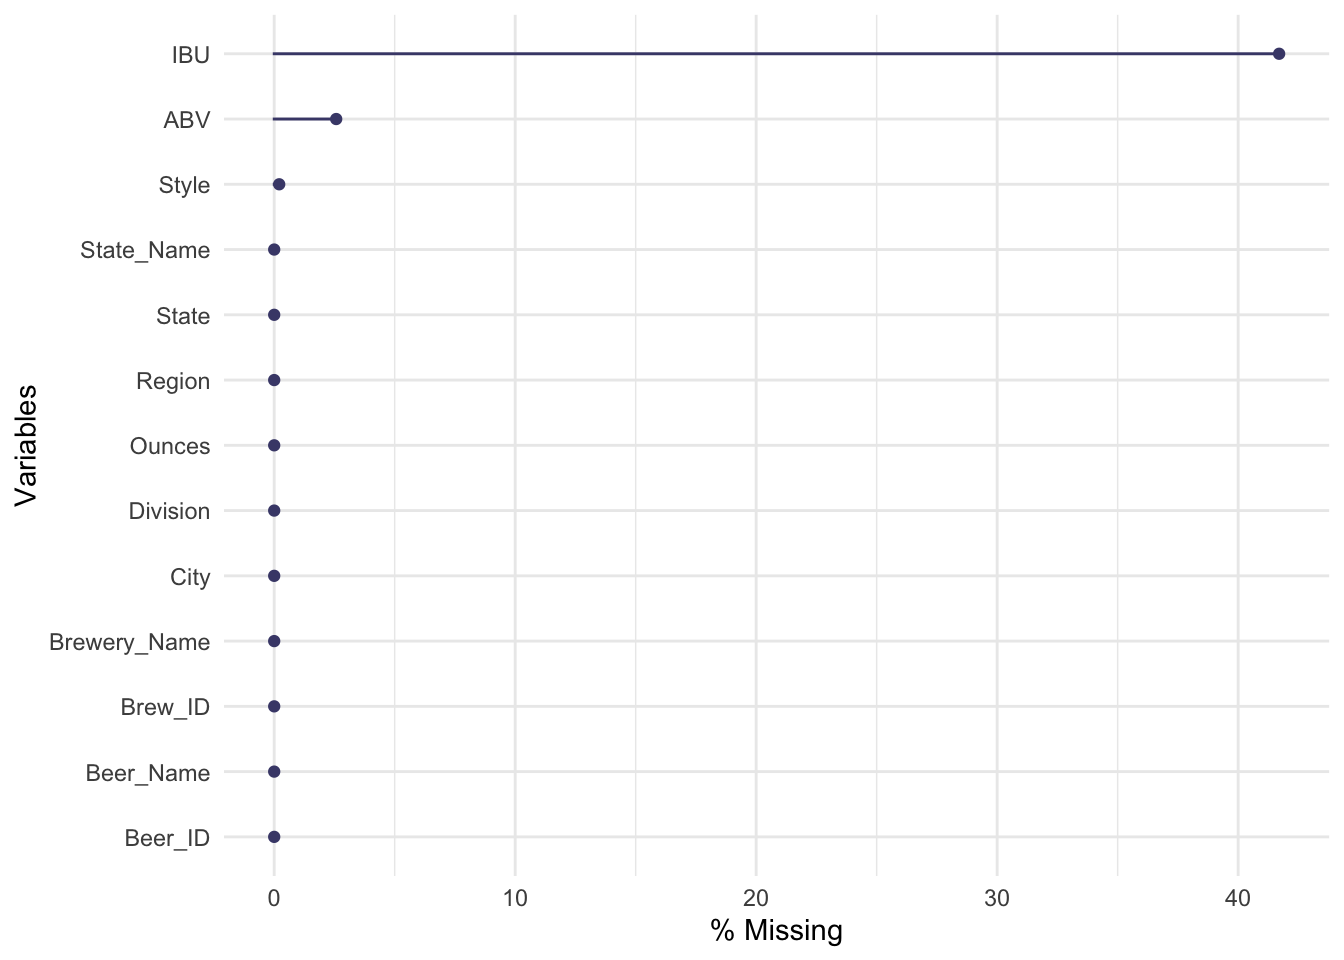
\includegraphics{bs_files/figure-latex/unnamed-chunk-4-1.pdf}

\#Code Chunk 5 \#\#This code computes the median alcohol content and
international bitterness unit for each state and plots them on a bar
chart to easily compare across sates. We have included a 5 number
summary to show the distribution across all states.

Median ABV: 5.6\% Median IBU: 35.00

\begin{Shaded}
\begin{Highlighting}[]
\CommentTok{\#bar chart of median ABV per state}
\NormalTok{bb }\SpecialCharTok{\%\textgreater{}\%} \FunctionTok{filter}\NormalTok{(}\SpecialCharTok{!}\FunctionTok{is.na}\NormalTok{(ABV)) }\SpecialCharTok{\%\textgreater{}\%}
   \FunctionTok{ggplot}\NormalTok{(}\FunctionTok{aes}\NormalTok{(State, ABV, }\AttributeTok{fill =}\NormalTok{ Region)) }\SpecialCharTok{+}
   \FunctionTok{geom\_bar}\NormalTok{(}\AttributeTok{stat =} \StringTok{\textquotesingle{}summary\textquotesingle{}}\NormalTok{, }\AttributeTok{fun =} \StringTok{\textquotesingle{}median\textquotesingle{}}\NormalTok{) }\SpecialCharTok{+}
   \FunctionTok{theme}\NormalTok{(}\AttributeTok{axis.text.x =} \FunctionTok{element\_text}\NormalTok{(}\AttributeTok{angle =} \DecValTok{90}\NormalTok{, }\AttributeTok{hjust =} \DecValTok{1}\NormalTok{))}\SpecialCharTok{+}
   \FunctionTok{ggtitle}\NormalTok{(}\StringTok{\textquotesingle{}Median ABV Comparison by State\textquotesingle{}}\NormalTok{)}
\end{Highlighting}
\end{Shaded}

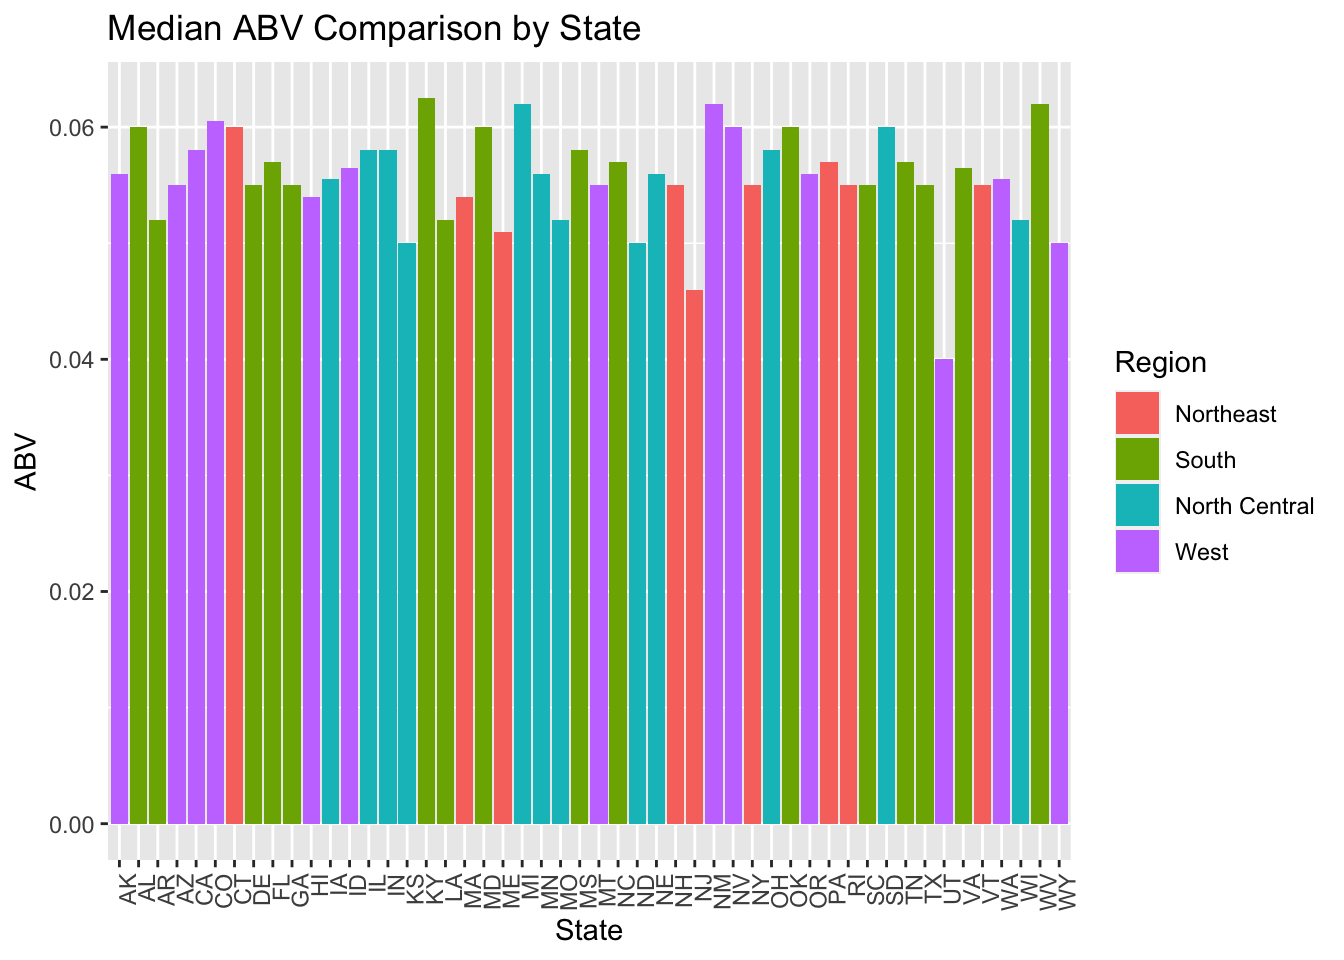
\includegraphics{bs_files/figure-latex/unnamed-chunk-5-1.pdf}

\begin{Shaded}
\begin{Highlighting}[]
\CommentTok{\#5 number summary of ABV}
\FunctionTok{summary}\NormalTok{(bb}\SpecialCharTok{$}\NormalTok{ABV)}
\end{Highlighting}
\end{Shaded}

\begin{verbatim}
##    Min. 1st Qu.  Median    Mean 3rd Qu.    Max.    NA's 
## 0.00100 0.05000 0.05600 0.05977 0.06700 0.12800      62
\end{verbatim}

\begin{Shaded}
\begin{Highlighting}[]
\CommentTok{\#bar chart of median IBU per state}
\NormalTok{bb }\SpecialCharTok{\%\textgreater{}\%} \FunctionTok{filter}\NormalTok{(}\SpecialCharTok{!}\FunctionTok{is.na}\NormalTok{(IBU)) }\SpecialCharTok{\%\textgreater{}\%}
   \FunctionTok{ggplot}\NormalTok{(}\FunctionTok{aes}\NormalTok{(State, IBU, }\AttributeTok{fill =}\NormalTok{ Region)) }\SpecialCharTok{+}
   \FunctionTok{geom\_bar}\NormalTok{(}\AttributeTok{stat =} \StringTok{\textquotesingle{}summary\textquotesingle{}}\NormalTok{, }\AttributeTok{fun=} \StringTok{\textquotesingle{}median\textquotesingle{}}\NormalTok{) }\SpecialCharTok{+}
   \FunctionTok{theme}\NormalTok{(}\AttributeTok{axis.text.x =} \FunctionTok{element\_text}\NormalTok{(}\AttributeTok{angle =} \DecValTok{90}\NormalTok{, }\AttributeTok{hjust =} \DecValTok{1}\NormalTok{))}\SpecialCharTok{+}
   \FunctionTok{ggtitle}\NormalTok{(}\StringTok{\textquotesingle{}Median IBU Comparison by State\textquotesingle{}}\NormalTok{)}
\end{Highlighting}
\end{Shaded}

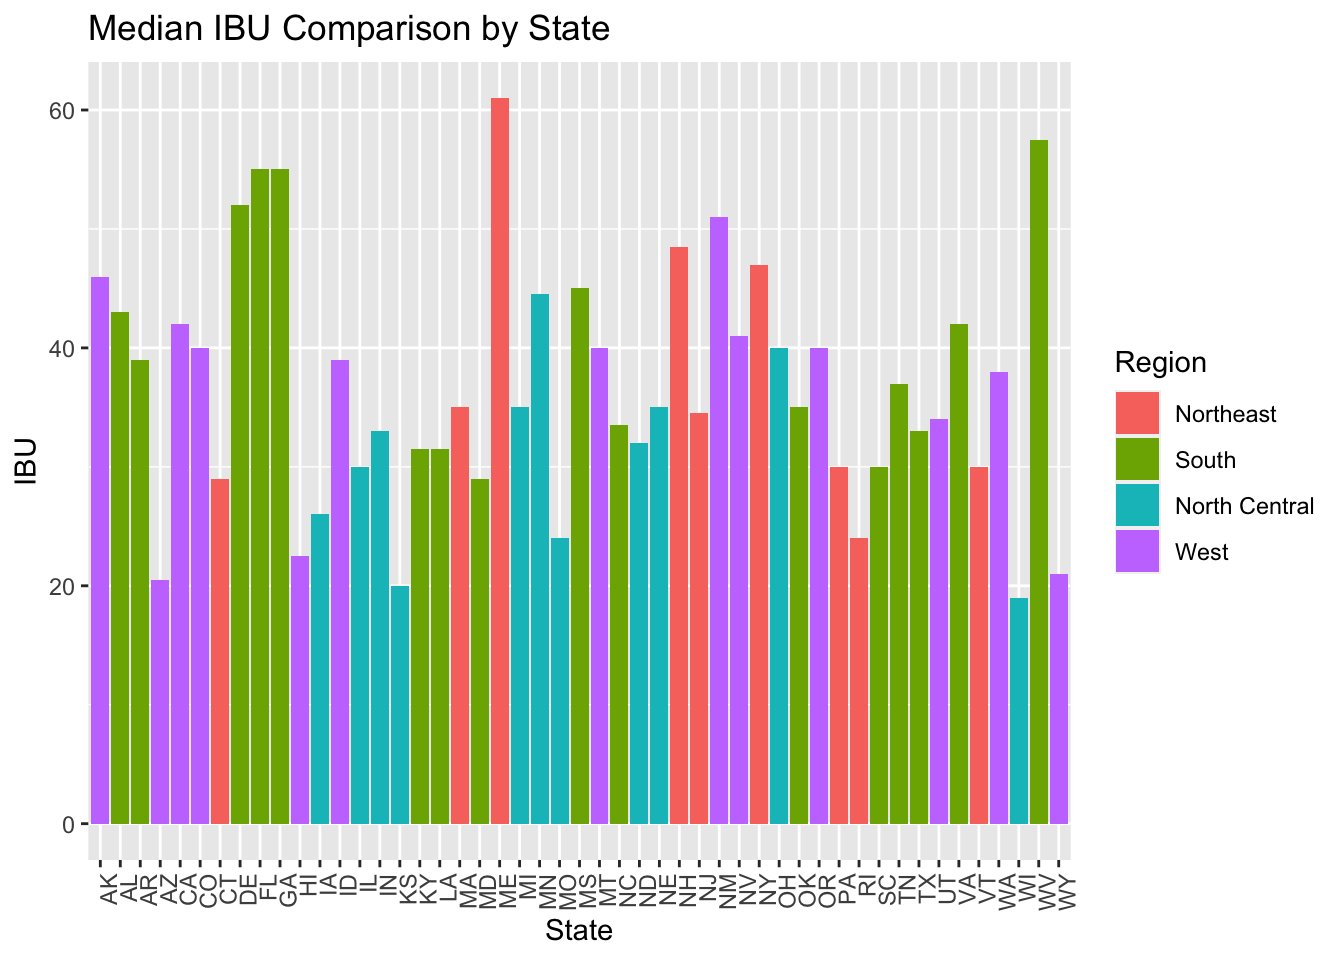
\includegraphics{bs_files/figure-latex/unnamed-chunk-5-2.pdf}

\begin{Shaded}
\begin{Highlighting}[]
\CommentTok{\#5 number summary of IBU}
\FunctionTok{summary}\NormalTok{(bb}\SpecialCharTok{$}\NormalTok{IBU)}
\end{Highlighting}
\end{Shaded}

\begin{verbatim}
##    Min. 1st Qu.  Median    Mean 3rd Qu.    Max.    NA's 
##    4.00   21.00   35.00   42.71   64.00  138.00    1005
\end{verbatim}

\#Code Chunk 6 \#\#In this code Chunk we determine which state has the
maximum alcoholic (ABV) beer and which state has the beer with the
highest IBU value.

Colorado has the beer with the highest ABV of 12.8 from Upslope Brewing.
Oregon has the beer with the highest IBU of 138 from Astoria Brewing.

\begin{Shaded}
\begin{Highlighting}[]
\CommentTok{\#finding record with maximum ABV}
\NormalTok{bb[}\FunctionTok{which.max}\NormalTok{(bb}\SpecialCharTok{$}\NormalTok{ABV),]}
\end{Highlighting}
\end{Shaded}

\begin{verbatim}
## # A tibble: 1 x 13
##   Brew_ID Brewery_Name  City   State Beer_Name  Beer_ID   ABV   IBU Style Ounces
##     <dbl> <chr>         <chr>  <chr> <chr>        <dbl> <dbl> <dbl> <chr>  <dbl>
## 1      52 Upslope Brew~ Bould~ CO    Lee Hill ~    2565 0.128    NA Quad~   19.2
## # ... with 3 more variables: State_Name <chr>, Region <fct>, Division <fct>
\end{verbatim}

\begin{Shaded}
\begin{Highlighting}[]
\CommentTok{\#finding record with maximum IBU}
\NormalTok{bb[}\FunctionTok{which.max}\NormalTok{(bb}\SpecialCharTok{$}\NormalTok{IBU),]}
\end{Highlighting}
\end{Shaded}

\begin{verbatim}
## # A tibble: 1 x 13
##   Brew_ID Brewery_Name  City   State Beer_Name Beer_ID   ABV   IBU Style  Ounces
##     <dbl> <chr>         <chr>  <chr> <chr>       <dbl> <dbl> <dbl> <chr>   <dbl>
## 1     375 Astoria Brew~ Astor~ OR    Bitter B~     980 0.082   138 Ameri~     12
## # ... with 3 more variables: State_Name <chr>, Region <fct>, Division <fct>
\end{verbatim}

\#Code Chunk 7 \#\#This code chunk calculates the summary statistics of
ABV and plots them broken out by Region.

The ABVs of beers in the data set range from 0.1\% to 12.8\% with an
average of 5.9\%. The majority of the beers in each region range from
5\% to 6.7\%.

\begin{Shaded}
\begin{Highlighting}[]
\CommentTok{\#obtain summary statistics of ABV}
\FunctionTok{summary}\NormalTok{(bb}\SpecialCharTok{$}\NormalTok{ABV)}
\end{Highlighting}
\end{Shaded}

\begin{verbatim}
##    Min. 1st Qu.  Median    Mean 3rd Qu.    Max.    NA's 
## 0.00100 0.05000 0.05600 0.05977 0.06700 0.12800      62
\end{verbatim}

\begin{Shaded}
\begin{Highlighting}[]
\CommentTok{\#box plot of ABV by region for analysis}
\NormalTok{bb }\SpecialCharTok{\%\textgreater{}\%}
   \FunctionTok{ggplot}\NormalTok{(}\FunctionTok{aes}\NormalTok{(ABV,Region))}\SpecialCharTok{+}
   \FunctionTok{geom\_boxplot}\NormalTok{(}\FunctionTok{aes}\NormalTok{(}\AttributeTok{fill =}\NormalTok{ Region))}
\end{Highlighting}
\end{Shaded}

\begin{verbatim}
## Warning: Removed 62 rows containing non-finite values (stat_boxplot).
\end{verbatim}

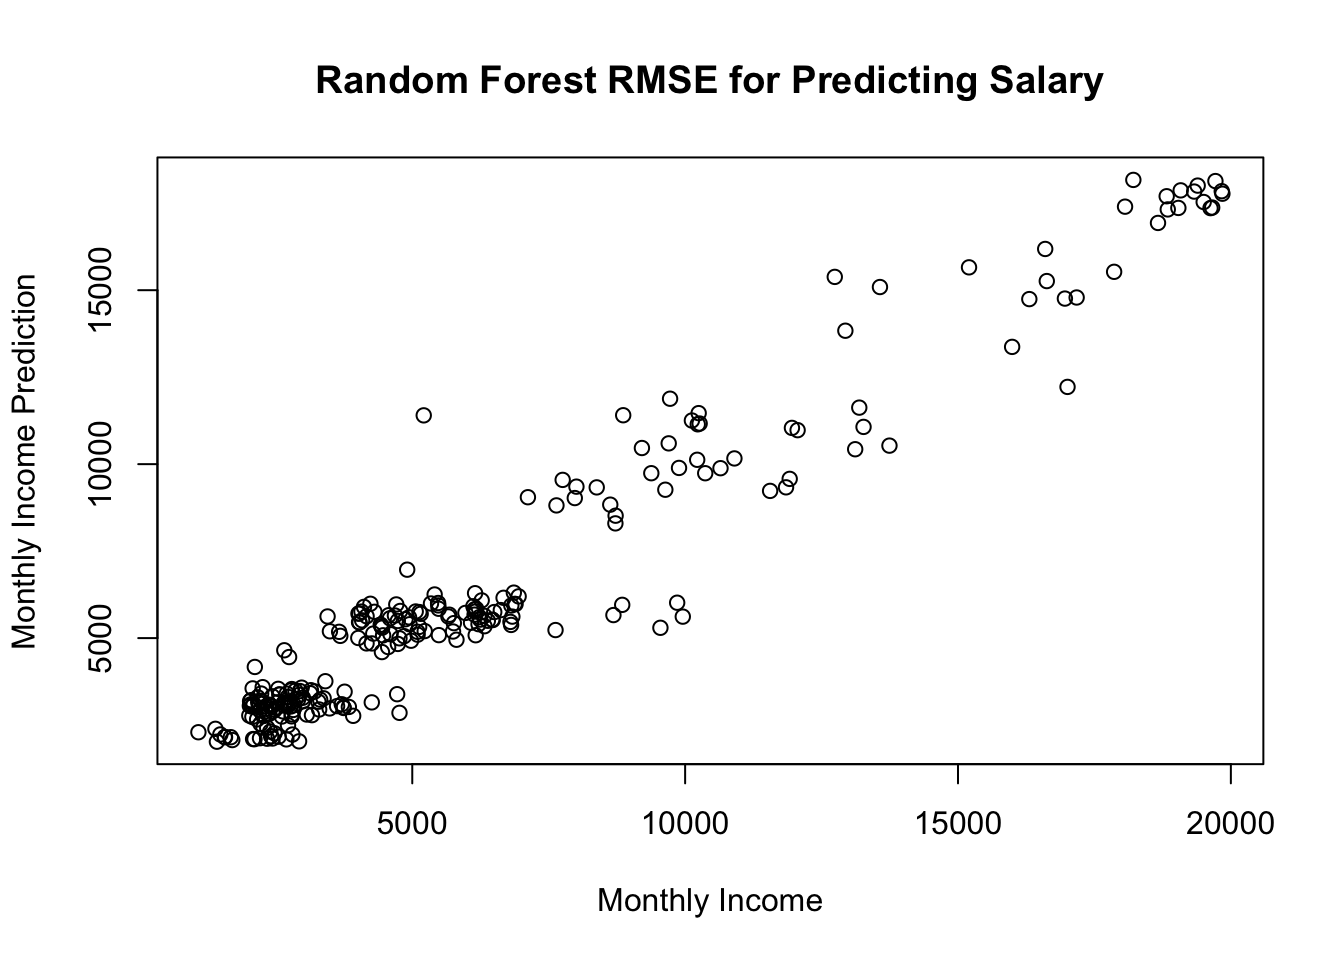
\includegraphics{bs_files/figure-latex/unnamed-chunk-7-1.pdf}

\#Code Chunk 8 \#\#The below code creates at scatter plot to calculate
the correlation between IBU and ABV by region.

There is a slight positive correlation between IBU and ABV. As ABV
increases IBU increases as well.

\begin{Shaded}
\begin{Highlighting}[]
\FunctionTok{library}\NormalTok{(ggthemes)}
\FunctionTok{library}\NormalTok{(ggpubr)}
\CommentTok{\#creating a scatter plot for relationship between IBU and ABV}
\CommentTok{\#adding pearson correlation information to determine relationship}
\CommentTok{\#breaking out graph by Region}
\NormalTok{bb }\SpecialCharTok{\%\textgreater{}\%}
   \FunctionTok{ggplot}\NormalTok{(}\FunctionTok{aes}\NormalTok{(ABV,IBU, }\AttributeTok{color =}\NormalTok{ Region)) }\SpecialCharTok{+}
   \FunctionTok{geom\_point}\NormalTok{(}\AttributeTok{position =} \StringTok{\textquotesingle{}jitter\textquotesingle{}}\NormalTok{)}\SpecialCharTok{+}
   \FunctionTok{geom\_smooth}\NormalTok{(}\AttributeTok{method =} \StringTok{\textquotesingle{}lm\textquotesingle{}}\NormalTok{)}\SpecialCharTok{+}
   \FunctionTok{stat\_cor}\NormalTok{(}\AttributeTok{method=}\StringTok{"pearson"}\NormalTok{, }\AttributeTok{label.x =} \DecValTok{0}\NormalTok{,}\AttributeTok{label.y =} \DecValTok{130}\NormalTok{)}\SpecialCharTok{+}
   \FunctionTok{ggtitle}\NormalTok{(}\StringTok{\textquotesingle{}Correlation of IBU and IPA in Beer by Region\textquotesingle{}}\NormalTok{)}\SpecialCharTok{+}
   \FunctionTok{facet\_wrap}\NormalTok{(}\SpecialCharTok{\textasciitilde{}}\NormalTok{Region)}\SpecialCharTok{+}
   \FunctionTok{theme\_minimal}\NormalTok{()}
\end{Highlighting}
\end{Shaded}

\begin{verbatim}
## `geom_smooth()` using formula 'y ~ x'
\end{verbatim}

\begin{verbatim}
## Warning: Removed 1005 rows containing non-finite values (stat_smooth).
\end{verbatim}

\begin{verbatim}
## Warning: Removed 1005 rows containing non-finite values (stat_cor).
\end{verbatim}

\begin{verbatim}
## Warning: Removed 1005 rows containing missing values (geom_point).
\end{verbatim}

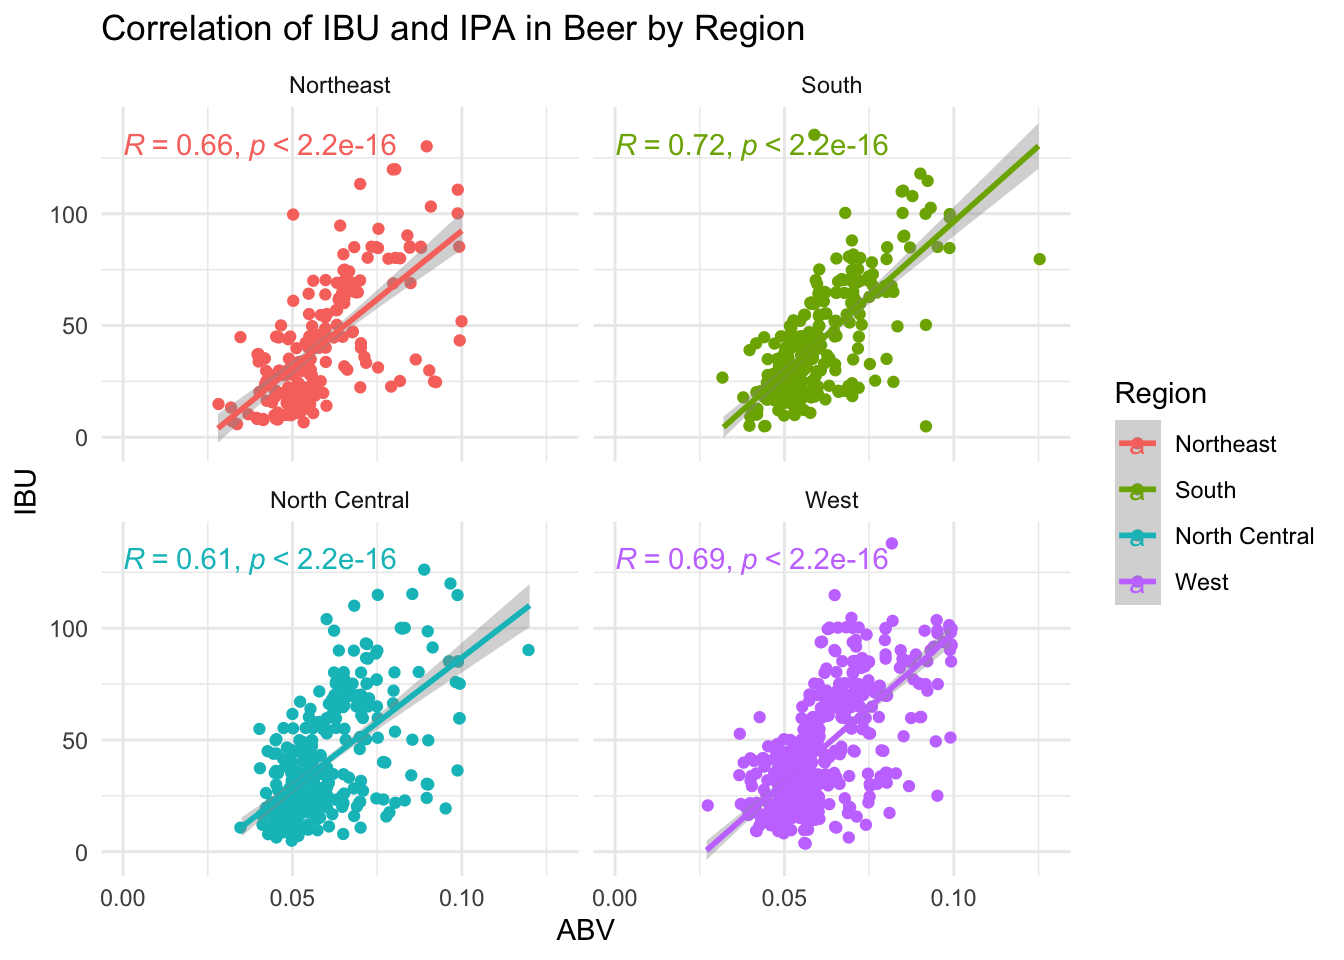
\includegraphics{bs_files/figure-latex/unnamed-chunk-8-1.pdf}

\#Code Chunk 9 \#\#The below code filters the overall data set to only
IPAs and Ales as well as imputes median values based on the style of the
beer. We then created a KNN model to predict if a beer is an IPA or Ale
based on IBU and ABV.

Using a KNN model, we were able to predict the style of beer with a
90.74\% accuracy.

\begin{Shaded}
\begin{Highlighting}[]
\FunctionTok{library}\NormalTok{(class)}
\FunctionTok{library}\NormalTok{(caret)}
\end{Highlighting}
\end{Shaded}

\begin{verbatim}
## Loading required package: lattice
\end{verbatim}

\begin{verbatim}
## 
## Attaching package: 'caret'
\end{verbatim}

\begin{verbatim}
## The following object is masked from 'package:purrr':
## 
##     lift
\end{verbatim}

\begin{Shaded}
\begin{Highlighting}[]
\FunctionTok{library}\NormalTok{(e1071)}

\FunctionTok{set.seed}\NormalTok{(}\DecValTok{25}\NormalTok{)}
\CommentTok{\#Filter down to Ale\textquotesingle{}s and IPA\textquotesingle{}s}
\NormalTok{bb\_knn }\OtherTok{=}\NormalTok{ bb }\SpecialCharTok{\%\textgreater{}\%}
   \FunctionTok{filter}\NormalTok{(}\FunctionTok{grepl}\NormalTok{(}\StringTok{\textquotesingle{}}\SpecialCharTok{\textbackslash{}\textbackslash{}}\StringTok{bAle}\SpecialCharTok{\textbackslash{}\textbackslash{}}\StringTok{b|}\SpecialCharTok{\textbackslash{}\textbackslash{}}\StringTok{bIPA}\SpecialCharTok{\textbackslash{}\textbackslash{}}\StringTok{b\textquotesingle{}}\NormalTok{,Style,}\AttributeTok{ignore.case =} \ConstantTok{TRUE}\NormalTok{))}

\CommentTok{\#create IPA/Ale column for analysis}
\NormalTok{bb\_knn}\SpecialCharTok{$}\NormalTok{IPA\_Ale }\OtherTok{=} \FunctionTok{as.character}\NormalTok{(}\FunctionTok{ifelse}\NormalTok{(}\FunctionTok{grepl}\NormalTok{(}\StringTok{\textquotesingle{}}\SpecialCharTok{\textbackslash{}\textbackslash{}}\StringTok{bIPA}\SpecialCharTok{\textbackslash{}\textbackslash{}}\StringTok{b\textquotesingle{}}\NormalTok{,bb\_knn}\SpecialCharTok{$}\NormalTok{Style,}\AttributeTok{ignore.case =} \ConstantTok{TRUE}\NormalTok{),}\StringTok{\textquotesingle{}IPA\textquotesingle{}}\NormalTok{,}\StringTok{\textquotesingle{}Ale\textquotesingle{}}\NormalTok{))}

\CommentTok{\#fixing NA values in data set}
\CommentTok{\#find mean to impute for NA values }
\NormalTok{abv\_mean }\OtherTok{=} \FunctionTok{aggregate}\NormalTok{(ABV }\SpecialCharTok{\textasciitilde{}}\NormalTok{ IPA\_Ale, bb\_knn, mean)}
\NormalTok{abv\_mean}
\end{Highlighting}
\end{Shaded}

\begin{verbatim}
##   IPA_Ale        ABV
## 1     Ale 0.05681330
## 2     IPA 0.06879286
\end{verbatim}

\begin{Shaded}
\begin{Highlighting}[]
\NormalTok{ibu\_mean }\OtherTok{=} \FunctionTok{aggregate}\NormalTok{(IBU }\SpecialCharTok{\textasciitilde{}}\NormalTok{ IPA\_Ale, bb\_knn, mean)}
\NormalTok{ibu\_mean}
\end{Highlighting}
\end{Shaded}

\begin{verbatim}
##   IPA_Ale      IBU
## 1     Ale 34.33333
## 2     IPA 71.94898
\end{verbatim}

\begin{Shaded}
\begin{Highlighting}[]
\CommentTok{\#mutate NA values from mean values}
\NormalTok{bb\_knn }\OtherTok{=}\NormalTok{ bb\_knn }\SpecialCharTok{\%\textgreater{}\%}
   \FunctionTok{mutate}\NormalTok{(}\AttributeTok{IBU =} \FunctionTok{ifelse}\NormalTok{(IPA\_Ale }\SpecialCharTok{==}\StringTok{\textquotesingle{}IPA\textquotesingle{}}\NormalTok{, }\FunctionTok{replace\_na}\NormalTok{(IBU,ibu\_mean[[}\DecValTok{2}\NormalTok{,}\DecValTok{2}\NormalTok{]]),}\FunctionTok{replace\_na}\NormalTok{(IBU,ibu\_mean[[}\DecValTok{1}\NormalTok{,}\DecValTok{2}\NormalTok{]])))}\SpecialCharTok{\%\textgreater{}\%}
   \FunctionTok{mutate}\NormalTok{(}\AttributeTok{ABV =} \FunctionTok{ifelse}\NormalTok{(IPA\_Ale }\SpecialCharTok{==}\StringTok{\textquotesingle{}IPA\textquotesingle{}}\NormalTok{, }\FunctionTok{replace\_na}\NormalTok{(ABV,abv\_mean[[}\DecValTok{2}\NormalTok{,}\DecValTok{2}\NormalTok{]]),}\FunctionTok{replace\_na}\NormalTok{(ABV,abv\_mean[[}\DecValTok{1}\NormalTok{,}\DecValTok{2}\NormalTok{]])))}

\CommentTok{\#check for NA values after imputation}
\FunctionTok{gg\_miss\_var}\NormalTok{(bb\_knn,}\AttributeTok{show\_pct =} \ConstantTok{TRUE}\NormalTok{)}
\end{Highlighting}
\end{Shaded}

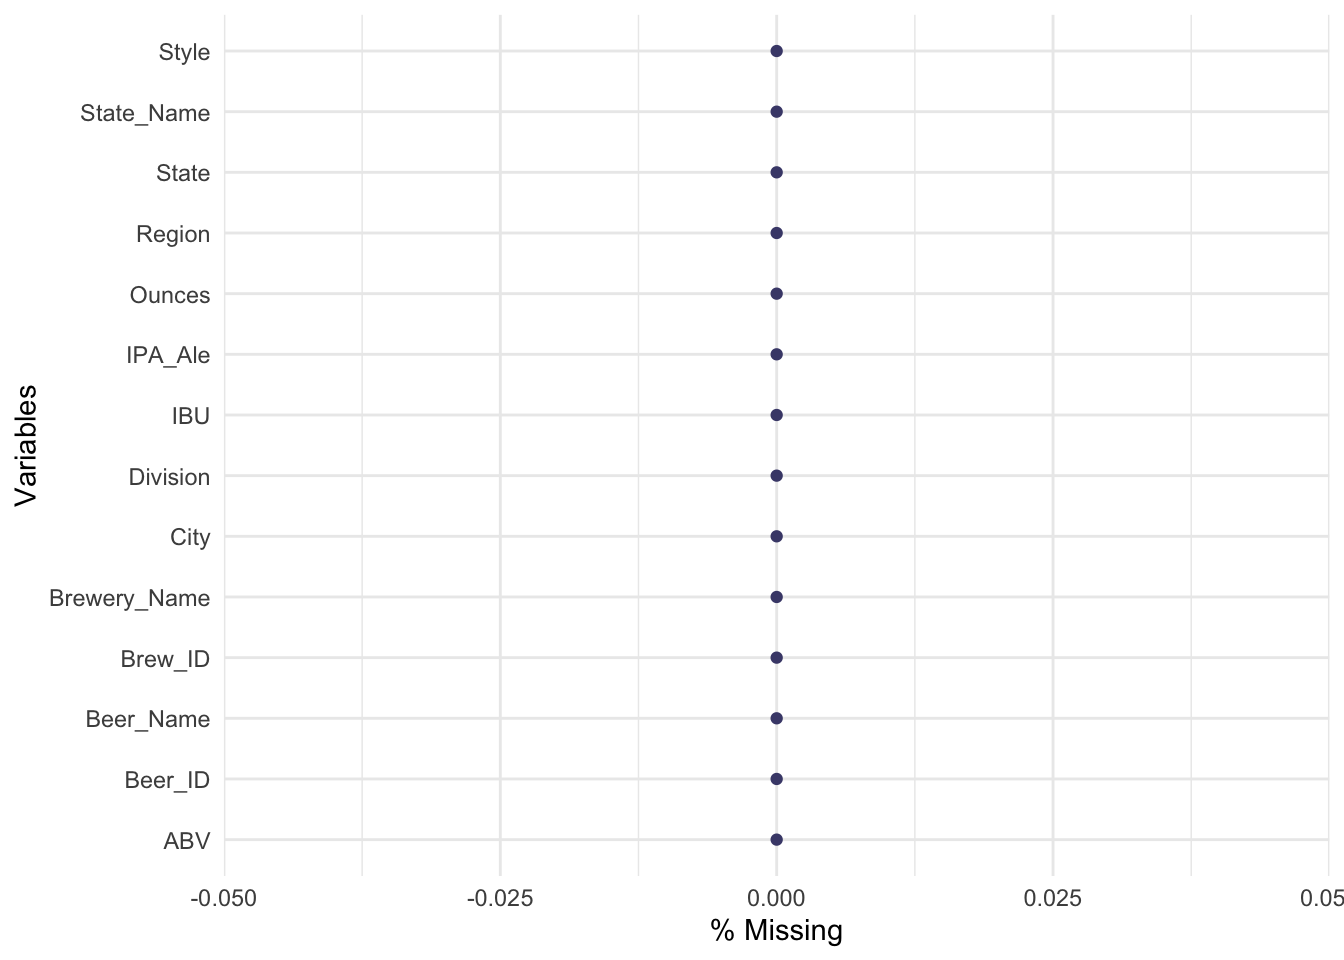
\includegraphics{bs_files/figure-latex/unnamed-chunk-9-1.pdf}

\begin{Shaded}
\begin{Highlighting}[]
\CommentTok{\#standardize IBU and ABV for knn model}
\NormalTok{bb\_knn}\SpecialCharTok{$}\NormalTok{Z\_IBU }\OtherTok{=} \FunctionTok{scale}\NormalTok{(bb\_knn}\SpecialCharTok{$}\NormalTok{IBU)}
\NormalTok{bb\_knn}\SpecialCharTok{$}\NormalTok{Z\_ABV }\OtherTok{=} \FunctionTok{scale}\NormalTok{(bb\_knn}\SpecialCharTok{$}\NormalTok{ABV)}


\CommentTok{\#creation of KNN model using leave one out method}
\NormalTok{classification }\OtherTok{=} \FunctionTok{knn.cv}\NormalTok{(bb\_knn[,}\FunctionTok{c}\NormalTok{(}\DecValTok{15}\NormalTok{,}\DecValTok{16}\NormalTok{)],bb\_knn}\SpecialCharTok{$}\NormalTok{IPA\_Ale,}\AttributeTok{prob =} \ConstantTok{TRUE}\NormalTok{, }\AttributeTok{k =} \DecValTok{10}\NormalTok{)}
\FunctionTok{table}\NormalTok{(classification,bb\_knn}\SpecialCharTok{$}\NormalTok{IPA\_Ale)}
\end{Highlighting}
\end{Shaded}

\begin{verbatim}
##               
## classification Ale IPA
##            Ale 894  74
##            IPA  69 497
\end{verbatim}

\begin{Shaded}
\begin{Highlighting}[]
\FunctionTok{confusionMatrix}\NormalTok{(}\FunctionTok{table}\NormalTok{(classification,bb\_knn}\SpecialCharTok{$}\NormalTok{IPA\_Ale))}
\end{Highlighting}
\end{Shaded}

\begin{verbatim}
## Confusion Matrix and Statistics
## 
##               
## classification Ale IPA
##            Ale 894  74
##            IPA  69 497
##                                           
##                Accuracy : 0.9068          
##                  95% CI : (0.8911, 0.9209)
##     No Information Rate : 0.6278          
##     P-Value [Acc > NIR] : <2e-16          
##                                           
##                   Kappa : 0.8002          
##                                           
##  Mcnemar's Test P-Value : 0.738           
##                                           
##             Sensitivity : 0.9283          
##             Specificity : 0.8704          
##          Pos Pred Value : 0.9236          
##          Neg Pred Value : 0.8781          
##              Prevalence : 0.6278          
##          Detection Rate : 0.5828          
##    Detection Prevalence : 0.6310          
##       Balanced Accuracy : 0.8994          
##                                           
##        'Positive' Class : Ale             
## 
\end{verbatim}

\#Code Chunk 10 \#\#In this code chunk we run and additional predictive
model called Naive Bayes to compare to our KNN model.

To find the most accurate model, we compared against a Naive Bayes model
which was slighly less accurate at predicting the beer style by 2\%.

\begin{Shaded}
\begin{Highlighting}[]
\CommentTok{\#NAIVE BAYES model to compare to KNN}
\CommentTok{\#set seed for reproducible results}
\FunctionTok{set.seed}\NormalTok{(}\DecValTok{4}\NormalTok{)}

\CommentTok{\#creating a 70/30 split for train and test data sets}
\NormalTok{trainIndices }\OtherTok{=} \FunctionTok{sample}\NormalTok{(}\FunctionTok{seq}\NormalTok{(}\DecValTok{1}\SpecialCharTok{:}\FunctionTok{length}\NormalTok{(bb\_knn}\SpecialCharTok{$}\NormalTok{IPA\_Ale)),}\FunctionTok{round}\NormalTok{(.}\DecValTok{7}\SpecialCharTok{*}\FunctionTok{length}\NormalTok{(bb\_knn}\SpecialCharTok{$}\NormalTok{IPA\_Ale)))}

\CommentTok{\#creating test and train data sets}
\NormalTok{train\_nb }\OtherTok{=}\NormalTok{ bb\_knn[trainIndices,]}
\NormalTok{test\_nb }\OtherTok{=}\NormalTok{ bb\_knn[}\SpecialCharTok{{-}}\NormalTok{trainIndices,]}

\CommentTok{\#running naive bayes model }
\NormalTok{model }\OtherTok{=} \FunctionTok{naiveBayes}\NormalTok{(train\_nb[,}\FunctionTok{c}\NormalTok{(}\DecValTok{15}\NormalTok{,}\DecValTok{16}\NormalTok{)],train\_nb}\SpecialCharTok{$}\NormalTok{IPA\_Ale)}
\FunctionTok{table}\NormalTok{(}\FunctionTok{predict}\NormalTok{(model,test\_nb[,}\FunctionTok{c}\NormalTok{(}\DecValTok{15}\NormalTok{,}\DecValTok{16}\NormalTok{)]),test\_nb}\SpecialCharTok{$}\NormalTok{IPA\_Ale)}
\end{Highlighting}
\end{Shaded}

\begin{verbatim}
##      
##       Ale IPA
##   Ale 259  28
##   IPA  23 150
\end{verbatim}

\begin{Shaded}
\begin{Highlighting}[]
\FunctionTok{confusionMatrix}\NormalTok{(}\FunctionTok{table}\NormalTok{(}\FunctionTok{predict}\NormalTok{(model,test\_nb[,}\FunctionTok{c}\NormalTok{(}\DecValTok{15}\NormalTok{,}\DecValTok{16}\NormalTok{)]),test\_nb}\SpecialCharTok{$}\NormalTok{IPA\_Ale))}
\end{Highlighting}
\end{Shaded}

\begin{verbatim}
## Confusion Matrix and Statistics
## 
##      
##       Ale IPA
##   Ale 259  28
##   IPA  23 150
##                                           
##                Accuracy : 0.8891          
##                  95% CI : (0.8568, 0.9163)
##     No Information Rate : 0.613           
##     P-Value [Acc > NIR] : <2e-16          
##                                           
##                   Kappa : 0.7651          
##                                           
##  Mcnemar's Test P-Value : 0.5754          
##                                           
##             Sensitivity : 0.9184          
##             Specificity : 0.8427          
##          Pos Pred Value : 0.9024          
##          Neg Pred Value : 0.8671          
##              Prevalence : 0.6130          
##          Detection Rate : 0.5630          
##    Detection Prevalence : 0.6239          
##       Balanced Accuracy : 0.8806          
##                                           
##        'Positive' Class : Ale             
## 
\end{verbatim}

\#Code Chunk 11 \#\#In this code section, we run our previous KNN model
90 times to determine the best parameters for our model.

In this section we ran the model 90 times to get the best parameter for
the model. When using the tuned model with a k=30 we were able to
accurately predict the style 92\% of the time.

\begin{Shaded}
\begin{Highlighting}[]
\FunctionTok{set.seed}\NormalTok{(}\DecValTok{25}\NormalTok{)}
\CommentTok{\#running KNN model 90 times to find best k parameter }
\NormalTok{accs }\OtherTok{=} \FunctionTok{data.frame}\NormalTok{(}\AttributeTok{accuracy =} \FunctionTok{numeric}\NormalTok{(}\DecValTok{90}\NormalTok{), }\AttributeTok{k =} \FunctionTok{numeric}\NormalTok{(}\DecValTok{90}\NormalTok{))}

\ControlFlowTok{for}\NormalTok{(i }\ControlFlowTok{in} \DecValTok{1}\SpecialCharTok{:}\DecValTok{90}\NormalTok{)}
\NormalTok{\{}
\NormalTok{   classification }\OtherTok{=} \FunctionTok{knn.cv}\NormalTok{(bb\_knn[,}\FunctionTok{c}\NormalTok{(}\DecValTok{15}\NormalTok{,}\DecValTok{16}\NormalTok{)],bb\_knn}\SpecialCharTok{$}\NormalTok{IPA\_Ale,}\AttributeTok{prob =} \ConstantTok{TRUE}\NormalTok{, }\AttributeTok{k =}\NormalTok{ i)}
   \FunctionTok{table}\NormalTok{(classification,bb\_knn}\SpecialCharTok{$}\NormalTok{IPA\_Ale)}
\NormalTok{   CM }\OtherTok{=} \FunctionTok{confusionMatrix}\NormalTok{(}\FunctionTok{table}\NormalTok{(classification,bb\_knn}\SpecialCharTok{$}\NormalTok{IPA\_Ale))}
\NormalTok{  accs}\SpecialCharTok{$}\NormalTok{accuracy[i] }\OtherTok{=}\NormalTok{ CM}\SpecialCharTok{$}\NormalTok{overall[}\DecValTok{1}\NormalTok{]}
\NormalTok{  accs}\SpecialCharTok{$}\NormalTok{k[i] }\OtherTok{=}\NormalTok{ i}
\NormalTok{\}}

\FunctionTok{plot}\NormalTok{(accs}\SpecialCharTok{$}\NormalTok{k,accs}\SpecialCharTok{$}\NormalTok{accuracy, }\AttributeTok{type =} \StringTok{"l"}\NormalTok{, }\AttributeTok{xlab =} \StringTok{"k"}\NormalTok{)}
\FunctionTok{abline}\NormalTok{(}\AttributeTok{v=}\NormalTok{accs}\SpecialCharTok{$}\NormalTok{k[}\FunctionTok{which.max}\NormalTok{(accs}\SpecialCharTok{$}\NormalTok{accuracy)], }\AttributeTok{col=}\StringTok{"red"}\NormalTok{)}
\end{Highlighting}
\end{Shaded}

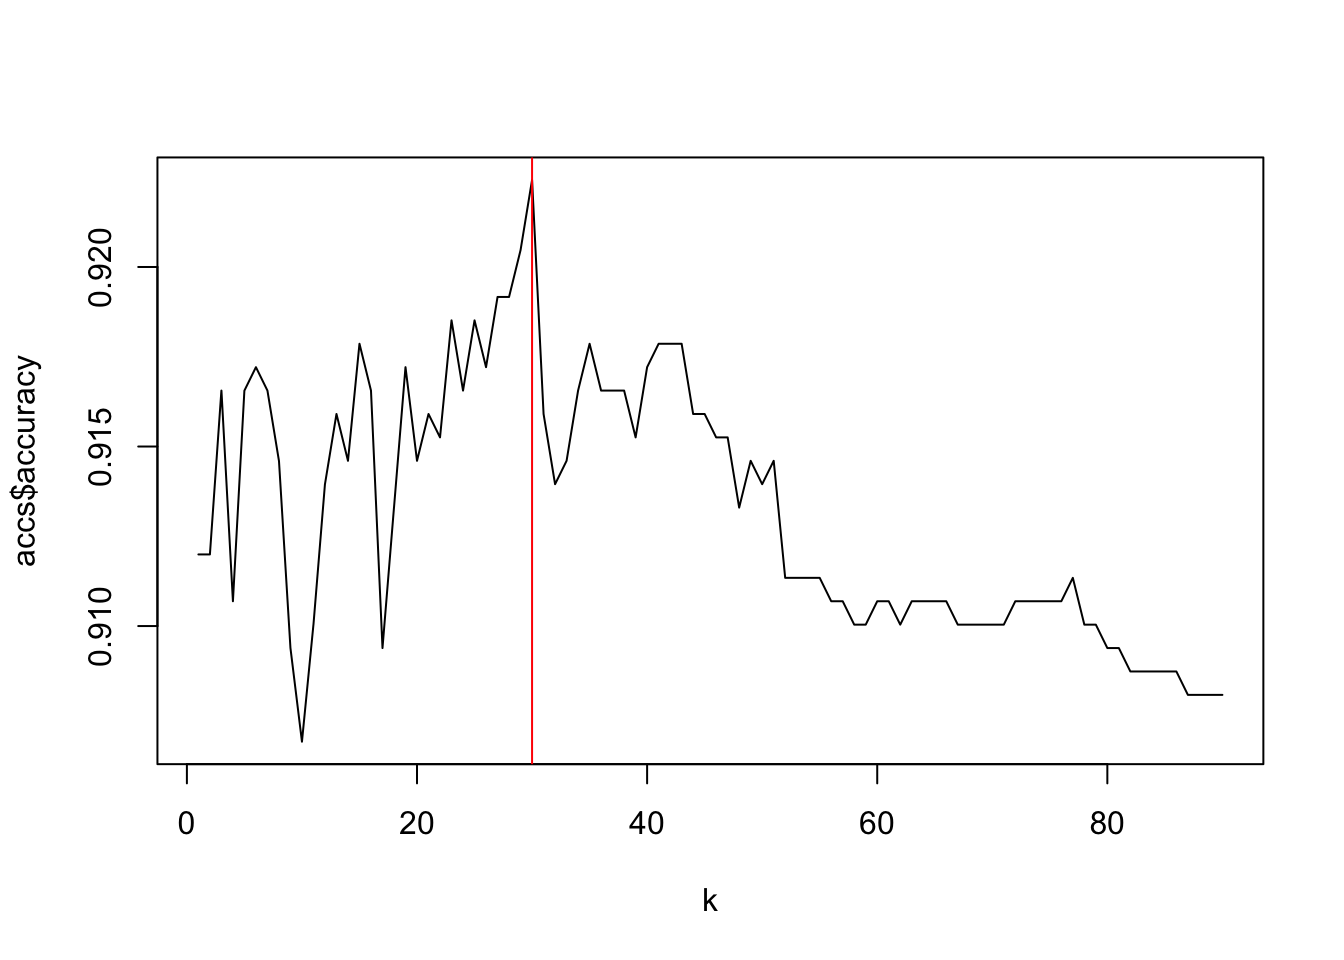
\includegraphics{bs_files/figure-latex/unnamed-chunk-11-1.pdf}

\begin{Shaded}
\begin{Highlighting}[]
\NormalTok{accs}\SpecialCharTok{$}\NormalTok{k[}\FunctionTok{which.max}\NormalTok{(accs}\SpecialCharTok{$}\NormalTok{accuracy)]}
\end{Highlighting}
\end{Shaded}

\begin{verbatim}
## [1] 30
\end{verbatim}

\begin{Shaded}
\begin{Highlighting}[]
\FunctionTok{set.seed}\NormalTok{(}\DecValTok{25}\NormalTok{)}
\CommentTok{\#use tuned parameter from code above}
\NormalTok{classification }\OtherTok{=} \FunctionTok{knn.cv}\NormalTok{(bb\_knn[,}\FunctionTok{c}\NormalTok{(}\DecValTok{15}\NormalTok{,}\DecValTok{16}\NormalTok{)],bb\_knn}\SpecialCharTok{$}\NormalTok{IPA\_Ale,}\AttributeTok{prob =} \ConstantTok{TRUE}\NormalTok{, }\AttributeTok{k =} \DecValTok{30}\NormalTok{)}
\FunctionTok{table}\NormalTok{(classification,bb\_knn}\SpecialCharTok{$}\NormalTok{IPA\_Ale)}
\end{Highlighting}
\end{Shaded}

\begin{verbatim}
##               
## classification Ale IPA
##            Ale 908  66
##            IPA  55 505
\end{verbatim}

\begin{Shaded}
\begin{Highlighting}[]
\FunctionTok{confusionMatrix}\NormalTok{(}\FunctionTok{table}\NormalTok{(classification,bb\_knn}\SpecialCharTok{$}\NormalTok{IPA\_Ale))}
\end{Highlighting}
\end{Shaded}

\begin{verbatim}
## Confusion Matrix and Statistics
## 
##               
## classification Ale IPA
##            Ale 908  66
##            IPA  55 505
##                                           
##                Accuracy : 0.9211          
##                  95% CI : (0.9065, 0.9341)
##     No Information Rate : 0.6278          
##     P-Value [Acc > NIR] : <2e-16          
##                                           
##                   Kappa : 0.8306          
##                                           
##  Mcnemar's Test P-Value : 0.3633          
##                                           
##             Sensitivity : 0.9429          
##             Specificity : 0.8844          
##          Pos Pred Value : 0.9322          
##          Neg Pred Value : 0.9018          
##              Prevalence : 0.6278          
##          Detection Rate : 0.5919          
##    Detection Prevalence : 0.6349          
##       Balanced Accuracy : 0.9137          
##                                           
##        'Positive' Class : Ale             
## 
\end{verbatim}

\#Code Chunk 12 In the below code, we join to another US data set to
plot a US heat map of the brewery count by state for easy analysis.

\begin{Shaded}
\begin{Highlighting}[]
\FunctionTok{library}\NormalTok{(maps)}
\end{Highlighting}
\end{Shaded}

\begin{verbatim}
## 
## Attaching package: 'maps'
\end{verbatim}

\begin{verbatim}
## The following object is masked from 'package:purrr':
## 
##     map
\end{verbatim}

\begin{Shaded}
\begin{Highlighting}[]
\FunctionTok{library}\NormalTok{(plotly)}
\end{Highlighting}
\end{Shaded}

\begin{verbatim}
## 
## Attaching package: 'plotly'
\end{verbatim}

\begin{verbatim}
## The following object is masked from 'package:ggplot2':
## 
##     last_plot
\end{verbatim}

\begin{verbatim}
## The following object is masked from 'package:stats':
## 
##     filter
\end{verbatim}

\begin{verbatim}
## The following object is masked from 'package:graphics':
## 
##     layout
\end{verbatim}

\begin{Shaded}
\begin{Highlighting}[]
\CommentTok{\#create heat map of breweries per state}

\NormalTok{states\_map }\OtherTok{=} \FunctionTok{map\_data}\NormalTok{(}\StringTok{"state"}\NormalTok{)}
\FunctionTok{names}\NormalTok{(states\_map)[}\DecValTok{5}\NormalTok{] }\OtherTok{=} \StringTok{\textquotesingle{}State\_Name\textquotesingle{}}
\NormalTok{states\_map }\OtherTok{=} \FunctionTok{left\_join}\NormalTok{(states\_map,state,}\AttributeTok{by=}\ConstantTok{NULL}\NormalTok{)}
\end{Highlighting}
\end{Shaded}

\begin{verbatim}
## Joining, by = "State_Name"
\end{verbatim}

\begin{Shaded}
\begin{Highlighting}[]
\NormalTok{states\_map }\OtherTok{=} \FunctionTok{left\_join}\NormalTok{(breweries, states\_map, }\AttributeTok{by =} \ConstantTok{NULL}\NormalTok{)}
\end{Highlighting}
\end{Shaded}

\begin{verbatim}
## Joining, by = "State"
\end{verbatim}

\begin{Shaded}
\begin{Highlighting}[]
\NormalTok{states\_map}
\end{Highlighting}
\end{Shaded}

\begin{verbatim}
## # A tibble: 223,088 x 12
##    Brew_ID Brewery_Name City  State  long   lat group order State_Name subregion
##      <dbl> <chr>        <chr> <chr> <dbl> <dbl> <dbl> <int> <chr>      <chr>    
##  1       1 NorthGate B~ Minn~ MN    -96.4  43.5    25  7047 minnesota  <NA>     
##  2       1 NorthGate B~ Minn~ MN    -96.4  43.9    25  7048 minnesota  <NA>     
##  3       1 NorthGate B~ Minn~ MN    -96.4  44.2    25  7049 minnesota  <NA>     
##  4       1 NorthGate B~ Minn~ MN    -96.4  44.5    25  7050 minnesota  <NA>     
##  5       1 NorthGate B~ Minn~ MN    -96.4  44.6    25  7051 minnesota  <NA>     
##  6       1 NorthGate B~ Minn~ MN    -96.4  44.8    25  7052 minnesota  <NA>     
##  7       1 NorthGate B~ Minn~ MN    -96.4  45.0    25  7053 minnesota  <NA>     
##  8       1 NorthGate B~ Minn~ MN    -96.4  45.3    25  7054 minnesota  <NA>     
##  9       1 NorthGate B~ Minn~ MN    -96.4  45.3    25  7055 minnesota  <NA>     
## 10       1 NorthGate B~ Minn~ MN    -96.4  45.3    25  7056 minnesota  <NA>     
## # ... with 223,078 more rows, and 2 more variables: Region <fct>,
## #   Division <fct>
\end{verbatim}

\begin{Shaded}
\begin{Highlighting}[]
\NormalTok{states\_map}
\end{Highlighting}
\end{Shaded}

\begin{verbatim}
## # A tibble: 223,088 x 12
##    Brew_ID Brewery_Name City  State  long   lat group order State_Name subregion
##      <dbl> <chr>        <chr> <chr> <dbl> <dbl> <dbl> <int> <chr>      <chr>    
##  1       1 NorthGate B~ Minn~ MN    -96.4  43.5    25  7047 minnesota  <NA>     
##  2       1 NorthGate B~ Minn~ MN    -96.4  43.9    25  7048 minnesota  <NA>     
##  3       1 NorthGate B~ Minn~ MN    -96.4  44.2    25  7049 minnesota  <NA>     
##  4       1 NorthGate B~ Minn~ MN    -96.4  44.5    25  7050 minnesota  <NA>     
##  5       1 NorthGate B~ Minn~ MN    -96.4  44.6    25  7051 minnesota  <NA>     
##  6       1 NorthGate B~ Minn~ MN    -96.4  44.8    25  7052 minnesota  <NA>     
##  7       1 NorthGate B~ Minn~ MN    -96.4  45.0    25  7053 minnesota  <NA>     
##  8       1 NorthGate B~ Minn~ MN    -96.4  45.3    25  7054 minnesota  <NA>     
##  9       1 NorthGate B~ Minn~ MN    -96.4  45.3    25  7055 minnesota  <NA>     
## 10       1 NorthGate B~ Minn~ MN    -96.4  45.3    25  7056 minnesota  <NA>     
## # ... with 223,078 more rows, and 2 more variables: Region <fct>,
## #   Division <fct>
\end{verbatim}

\begin{Shaded}
\begin{Highlighting}[]
\NormalTok{state\_heat }\OtherTok{=} \FunctionTok{left\_join}\NormalTok{(state,brew\_cnt, }\AttributeTok{by =} \ConstantTok{NULL}\NormalTok{)}
\end{Highlighting}
\end{Shaded}

\begin{verbatim}
## Joining, by = "State"
\end{verbatim}

\begin{Shaded}
\begin{Highlighting}[]
\CommentTok{\#merging brewery count to map data}
\NormalTok{states\_map }\OtherTok{=} \FunctionTok{left\_join}\NormalTok{(states\_map,state\_heat,}\AttributeTok{by=} \ConstantTok{NULL}\NormalTok{)}
\end{Highlighting}
\end{Shaded}

\begin{verbatim}
## Joining, by = c("State", "State_Name", "Region", "Division")
\end{verbatim}

\begin{Shaded}
\begin{Highlighting}[]
\NormalTok{states\_map}
\end{Highlighting}
\end{Shaded}

\begin{verbatim}
## # A tibble: 227,616 x 13
##    Brew_ID Brewery_Name City  State  long   lat group order State_Name subregion
##      <dbl> <chr>        <chr> <chr> <dbl> <dbl> <dbl> <int> <chr>      <chr>    
##  1       1 NorthGate B~ Minn~ MN    -96.4  43.5    25  7047 minnesota  <NA>     
##  2       1 NorthGate B~ Minn~ MN    -96.4  43.9    25  7048 minnesota  <NA>     
##  3       1 NorthGate B~ Minn~ MN    -96.4  44.2    25  7049 minnesota  <NA>     
##  4       1 NorthGate B~ Minn~ MN    -96.4  44.5    25  7050 minnesota  <NA>     
##  5       1 NorthGate B~ Minn~ MN    -96.4  44.6    25  7051 minnesota  <NA>     
##  6       1 NorthGate B~ Minn~ MN    -96.4  44.8    25  7052 minnesota  <NA>     
##  7       1 NorthGate B~ Minn~ MN    -96.4  45.0    25  7053 minnesota  <NA>     
##  8       1 NorthGate B~ Minn~ MN    -96.4  45.3    25  7054 minnesota  <NA>     
##  9       1 NorthGate B~ Minn~ MN    -96.4  45.3    25  7055 minnesota  <NA>     
## 10       1 NorthGate B~ Minn~ MN    -96.4  45.3    25  7056 minnesota  <NA>     
## # ... with 227,606 more rows, and 3 more variables: Region <fct>,
## #   Division <fct>, Brewery_Count <int>
\end{verbatim}

\begin{Shaded}
\begin{Highlighting}[]
\NormalTok{states\_map }\SpecialCharTok{\%\textgreater{}\%}
   \FunctionTok{ggplot}\NormalTok{(}\FunctionTok{aes}\NormalTok{(}\AttributeTok{x=}\NormalTok{long,}\AttributeTok{y=}\NormalTok{lat,}\AttributeTok{group=}\NormalTok{group))}\SpecialCharTok{+}
   \FunctionTok{geom\_polygon}\NormalTok{(}\FunctionTok{aes}\NormalTok{(}\AttributeTok{fill =}\NormalTok{ Brewery\_Count))}\SpecialCharTok{+}
   \FunctionTok{geom\_path}\NormalTok{()}\SpecialCharTok{+} 
   \FunctionTok{scale\_fill\_gradientn}\NormalTok{(}\AttributeTok{colours=}\FunctionTok{rev}\NormalTok{(}\FunctionTok{heat.colors}\NormalTok{(}\DecValTok{10}\NormalTok{)),}\AttributeTok{na.value=}\StringTok{"grey90"}\NormalTok{)}\SpecialCharTok{+}
   \FunctionTok{ggtitle}\NormalTok{(}\StringTok{"Breweries by State"}\NormalTok{)}\SpecialCharTok{+}
   \FunctionTok{labs}\NormalTok{(}\AttributeTok{color=}\StringTok{\textquotesingle{}Number of Breweries\textquotesingle{}}\NormalTok{)}\SpecialCharTok{+}
   \FunctionTok{coord\_map}\NormalTok{(}\StringTok{\textquotesingle{}bonne\textquotesingle{}}\NormalTok{,}\AttributeTok{parameters =} \FloatTok{41.6}\NormalTok{)}\SpecialCharTok{+}
   \FunctionTok{theme}\NormalTok{(}\AttributeTok{axis.text=} \FunctionTok{element\_blank}\NormalTok{(),}
         \AttributeTok{axis.title =} \FunctionTok{element\_blank}\NormalTok{(),}
         \AttributeTok{axis.ticks =} \FunctionTok{element\_blank}\NormalTok{())}
\end{Highlighting}
\end{Shaded}

\begin{verbatim}
## Warning: Removed 11 row(s) containing missing values (geom_path).
\end{verbatim}

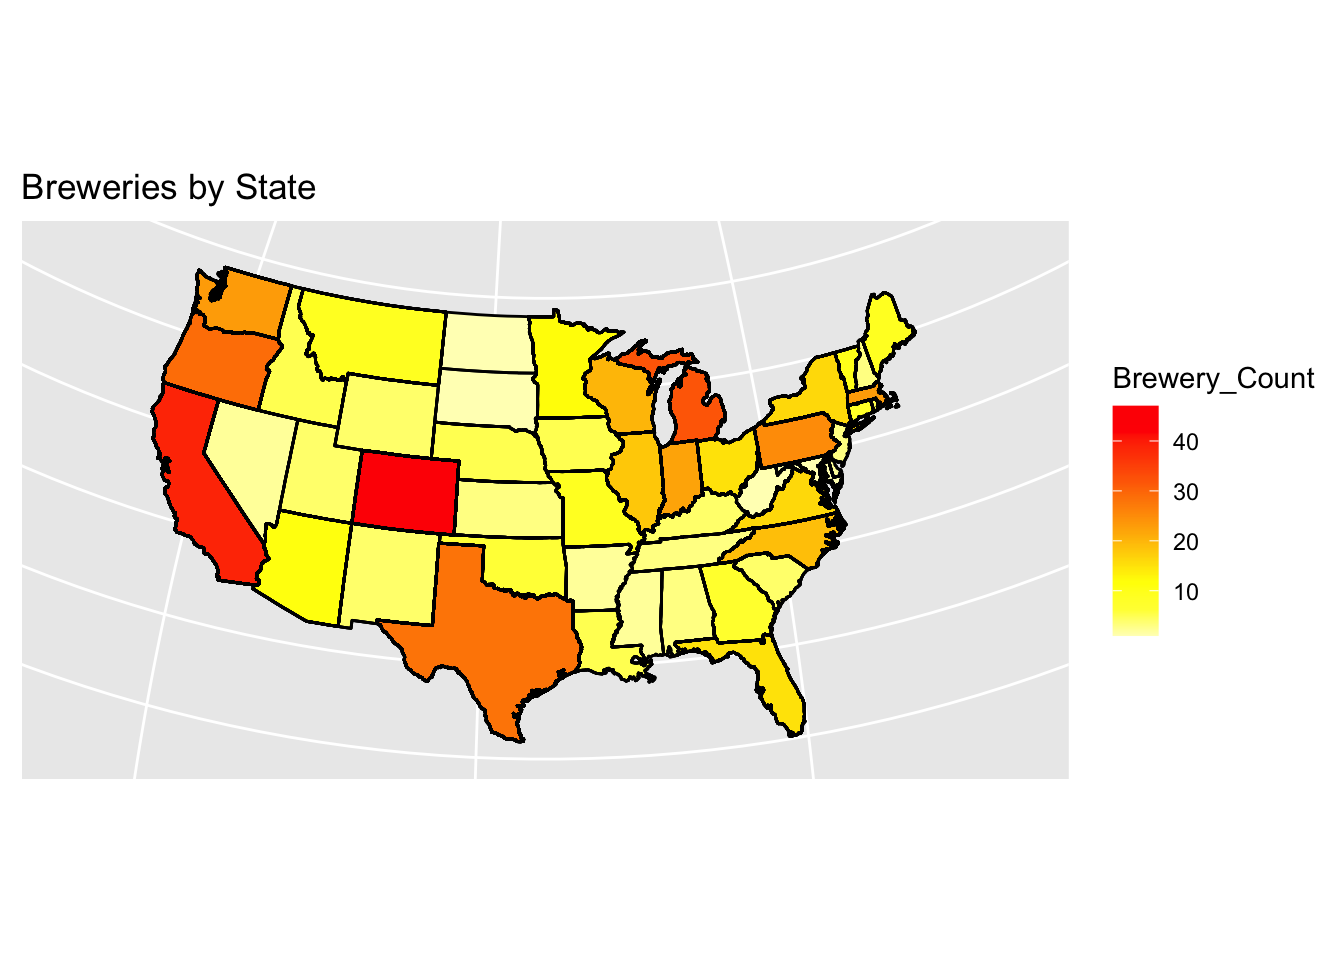
\includegraphics{bs_files/figure-latex/unnamed-chunk-12-1.pdf}

\#Code Chuck 13 This code creates a bar graph of the number of breweries
in each state ordered descending

\begin{Shaded}
\begin{Highlighting}[]
\CommentTok{\#creates bar chart for brewery count in each state}
\CommentTok{\#filtering out duplicate MD row}
\NormalTok{brew\_cnt\_bar }\OtherTok{=} \FunctionTok{left\_join}\NormalTok{(brew\_cnt,state,}\AttributeTok{by=}\ConstantTok{NULL}\NormalTok{)}
\end{Highlighting}
\end{Shaded}

\begin{verbatim}
## Joining, by = "State"
\end{verbatim}

\begin{Shaded}
\begin{Highlighting}[]
\NormalTok{brew\_cnt\_bar }\OtherTok{=}\NormalTok{brew\_cnt\_bar }\SpecialCharTok{\%\textgreater{}\%} \FunctionTok{filter}\NormalTok{(State }\SpecialCharTok{!=}\StringTok{\textquotesingle{}MD\textquotesingle{}}\SpecialCharTok{|}\NormalTok{Brewery\_Count }\SpecialCharTok{!=} \DecValTok{1}\NormalTok{)}


\NormalTok{brew\_cnt\_bar }\SpecialCharTok{\%\textgreater{}\%}
   \FunctionTok{ggplot}\NormalTok{(}\FunctionTok{aes}\NormalTok{(Brewery\_Count,}\FunctionTok{reorder}\NormalTok{(State,Brewery\_Count),}\AttributeTok{fill =}\NormalTok{ Region)) }\SpecialCharTok{+}
   \FunctionTok{geom\_col}\NormalTok{()}\SpecialCharTok{+}
   \FunctionTok{ggtitle}\NormalTok{(}\StringTok{\textquotesingle{}Number of Breweries in Each State\textquotesingle{}}\NormalTok{)}\SpecialCharTok{+}
   \FunctionTok{xlab}\NormalTok{(}\StringTok{\textquotesingle{}Number of Breweries\textquotesingle{}}\NormalTok{)}\SpecialCharTok{+}
   \FunctionTok{ylab}\NormalTok{(}\StringTok{\textquotesingle{}State\textquotesingle{}}\NormalTok{)}\SpecialCharTok{+}
   \FunctionTok{geom\_text}\NormalTok{(}\FunctionTok{aes}\NormalTok{(}\AttributeTok{label=}\NormalTok{Brewery\_Count),}\AttributeTok{hjust=}\DecValTok{1}\NormalTok{)}
\end{Highlighting}
\end{Shaded}

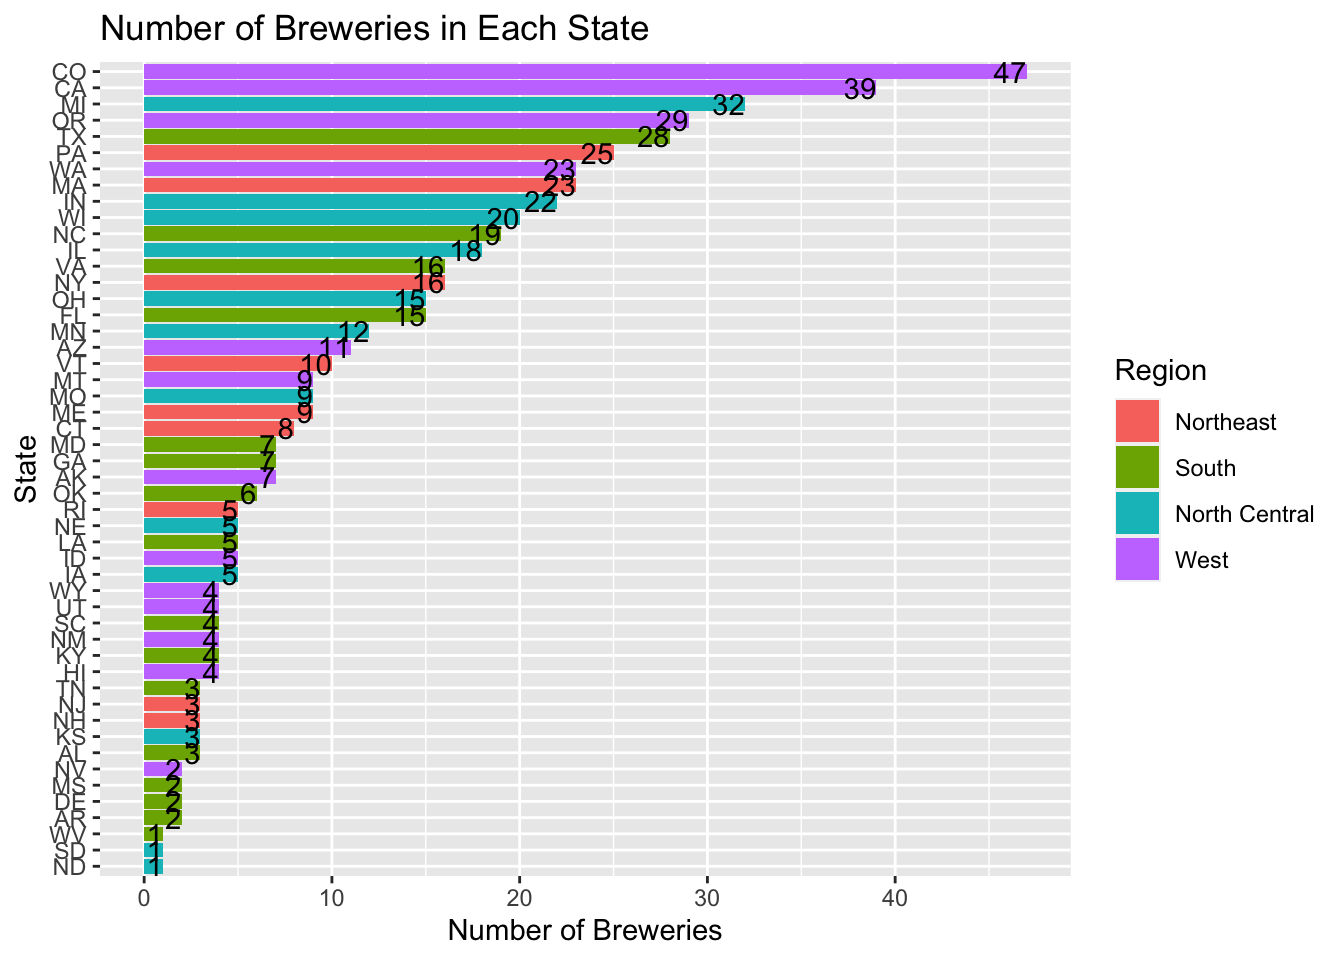
\includegraphics{bs_files/figure-latex/unnamed-chunk-13-1.pdf}

\end{document}
